\documentclass{beamer}

\usepackage{amsmath,amsthm,amssymb}
\usepackage{tikz}

\usetikzlibrary{positioning}

\beamertemplatenavigationsymbolsempty
\useoutertheme{split}
\useinnertheme{rounded}

\newcommand{\ite}[3]{(#1 ~\tikz[baseline] \draw[->, -stealth] (0ex,.5ex)--(2ex,.5ex);~ #2 , #3)}

\def\checkmark{\tikz\fill[scale=0.4](0,.35) -- (.25,0) -- (1,.7) -- (.25,.15) -- cycle;}

\tikzset{onslide/.code args={<#1>#2}{%
  \only<#1>{\pgfkeysalso{#2}} % \pgfkeysalso doesn't change the path
}}

\tikzstyle{highlight}=[draw=gray,fill=black,text=white]

\begin{document}

\title[Efficiently representing FACT using BDDs] % (optional, only for long titles)
{Efficiently representing the integer factorization problem using binary decision diagrams}
\subtitle{A reduction of FACT to BDD SAT}
\author[David Skidmore] % (optional, for multiple authors)
{David Skidmore}
\institute[Utah State University] % (optional)
{
Department of Mathematics and Statistics\\
Utah State University
}
\date[27 April 2017] % (optional)
{27 April 2017}

\maketitle

\section[Boolean functions]{Boolean functions}
\begin{frame}
\frametitle{Boolean functions}
\framesubtitle{for this presentation}

A \textit{boolean function} is a $\{0,1\}$-valued function in a finite number of $\{0,1\}$-valued (boolean) variables.
\end{frame}

\subsection[NOT]{NOT}
\begin{frame}
\begin{example}
The unary operation $\lnot$ (negation, boolean NOT) is defined by
\begin{center}
\begin{array}{c|c}
x & \lnot x\\
\hline
0 & 1 \\
1 & 0
\end{array}
\end{center}
It is common to use $\overline{x}$ to denote $\lnot x$.
\end{example}
\end{frame}

\subsection[AND]{AND}
\begin{frame}
\begin{example}
The binary operation $\land$ (conjunction, boolean AND, multiplication) is defined by
\begin{center}
\begin{array}{c|c|c}
x & y & x \land y \\
\hline
0 & 0 & 0 \\
0 & 1 & 0 \\
1 & 0 & 0 \\
1 & 1 & 1
\end{array}
\end{center}
It is common to use $xy$ to denote $x \land y$.
\end{example}
\end{frame}

\subsection[OR]{OR}
\begin{frame}
\begin{example}
The binary operation $\lor$ (disjunction, boolean OR) is defined by
\begin{center}
\begin{array}{c|c|c}
x & y & x \lor y \\
\hline
0 & 0 & 0 \\
0 & 1 & 1 \\
1 & 0 & 1 \\
1 & 1 & 1
\end{array}
\end{center}
\end{example}
\end{frame}

\subsection[XOR]{XOR}
\begin{frame}
\begin{example}
The binary operation $\oplus$ (exclusive disjunction, boolean XOR, modulo-$2$ additon) is defined by
\begin{center}
\begin{array}{c|c|c}
x & y & x \oplus y \\
\hline
0 & 0 & 0 \\
0 & 1 & 1 \\
1 & 0 & 1 \\
1 & 1 & 0
\end{array}
\end{center}
\end{example}
\end{frame}

\section[FACT]{FACT}
\begin{frame}
\frametitle{The integer factorization problem (FACT)}
Given a positive integer $a>1$, find positive integers $x,y>1$ such that
$$xy = a.$$
If no such $x$ and $y$ exist then $a$ is \textit{prime}, otherwise $a$ is \textit{composite}, $x$ and $y$ are \textit{factors} of $a$, and $xy$ is a \textit{factorization} of $a$.
\end{frame}

\subsection[Representing FACT]{Representing FACT}
\begin{frame}
\frametitle{Representing FACT with boolean functions}
Fix a positive integer $n$. For each nonnegative integer $m$ there is a boolean function $f_m : \{0,1\}^{2n} \to \{0,1\}$ such that $f_m(x_0,x_1,\dots,x_{n-1},y_0,y_1,\dots,y_{n-1})$ (represented by $f_m(\vec{x},\vec{y})$) gives the the coefficient of $2^m$ in the binary expansion of the product
$$(x_0 + 2x_1 + \dots + 2^{n-1}x_{n-1})(y_0 + 2y_1 + \dots + 2^{n-1}y_{n-1}).$$
\end{frame}

\subsection[Single]{Single}
\begin{frame}
Let $a>1$ be a positive integer with binary expansion $a_0 + 2a_1 + \dots + 2^{n-1}a_{n-1}$. Every factorization of $a$ corresponds to a solution of
$$F_a(\vec{x},\vec{y}) = 1$$
where
$$F_a(\vec{x},\vec{y}) = \prod_{m=0}^{2n-1}[1 \oplus a_m \oplus f_m(\vec{x},\vec{y})],$$
and if $m \geq n$ then let $a_m=0.$
\end{frame}

\subsection[System]{System}
\begin{frame}
$F_a(\vec{x},\vec{y})=1$ is equivalent to the system $S_a$,
\begin{align*}
a_0 \oplus f_0(\vec{x},\vec{y}) &= 0  \\
a_1 \oplus f_1(\vec{x},\vec{y}) &= 0  \\
 &\vdots \\
a_{n-1} \oplus f_{n-1}(\vec{x},\vec{y}) &= 0 \\
f_{n}(\vec{x},\vec{y}) &= 0 \\
 &\vdots \\
f_{2n-1}(\vec{x},\vec{y}) &= 0 
\end{align}
\end{frame}

\section[Boolean formulae]{Boolean formulae}
\begin{frame}
\frametitle{Boolean formulae}
A \textit{boolean formula} is a labeled directed rooted tree representing a mathematical term built from some collection of constant symbols $\{0,1\}$, and variable and operator symbols corresponding to boolean variables and functions.
\end{frame}

%\begin{frame}
%The leaves of a boolean formula are labeled by constants or variables. The inner vertices are labeled by operator symbols and have indegree equal to the arity of the function corresponding to its label.
%\end{frame}

\begin{frame}
\begin{example}
\begin{description}
\item [Formula:] $((w \land x) \lor ( (\lnot y) \lor x) )$
\end{description}
\begin{center}
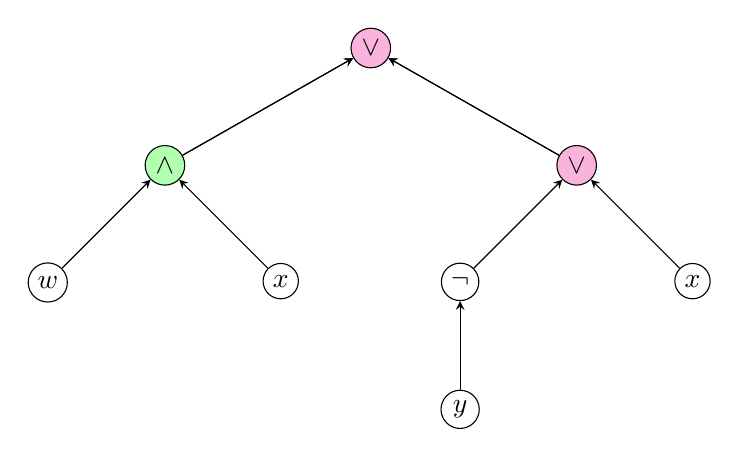
\begin{tikzpicture}[
node distance = 32pt and 64pt,
inner/.style={circle, draw=black, inner sep = 2pt, minimum size = 2pt},
terminal/.style={rectangle, draw=black, inner sep = 2pt, minimum size=2pt},
low/.style ={-stealth,dashed,red},
high/.style = {-stealth, solid,cyan}]

\node[inner, fill=magenta!30] (1) {$\lor$};
\node[inner, fill=green!30] (2) [below left = of 1] {$\land$};
\node[inner, fill=magenta!30] (3) [below right = of 1] {$\lor$};

\node[inner] (6) [below left = 32pt and 32pt of 3] {$\lnot$};

\node[inner] (4) [below left = 32pt and 32pt of 2] {$w$};
\node[inner] (5) [below right = 32pt and 32pt of 2] {$x$};

\node[inner] (7) [below right = 32pt and 32pt of 3] {$x$};
\node[inner] (8) [below =of 6] {$y$};

\draw[->,-stealth](2)--(1);
\draw[->,-stealth](2)--(1);

\draw[->,-stealth](3)--(1);
\draw[->,-stealth](3)--(1);

\draw[->,-stealth](4)--(2);
\draw[->,-stealth](5)--(2);

\draw[->,-stealth](6)--(3);
\draw[->,-stealth](7)--(3);

\draw[->,-stealth](8)--(6);
\end{tikzpicture}
\end{center}
\end{example}
\end{frame}

%\begin{frame}
%\begin{itemize}
%\item Using trees instead of strings is to ignore differences in notation we don't care about. For example, infix notation $(x \lor y)$ versus functional notation $\lor(x,y)$, although different strings they both correspond to the tree,

%\item Commonly refer to a mathematical term corresponding to a specific boolean formula as a boolean formula itself.

%\item For a given set of boolean functions $\Omega$ and variables $X$, a (boolean) \textit{formula over the basis $\Omega$ in the variables $X$} refers to a formula whose leaf labels are restricted to constants and $X$ and whose inner node labels are restricted to $\Omega$.
%\end{itemize}
%\end{frame}

%\subsection[Notation]{Notation}
%\begin{frame}
%\frametitle{Notation}
%\begin{itemize}
%\item It is common to omit the outermost pair of parenthesis from a string representing a boolean formula.
%\pause
%\item For a symbol $\phi$ which is not a constant or variable symbol, a particular boolean formula in finite number of variables $\{x_1,\dots,x_n\}$ may be referred to by $\phi(x_1,\dots,x_n)$.
%\end{itemize}
%\end{frame}

\subsection[func \gets form]{func \gets form}
%\begin{frame}
%\frametitle{Boolean functions from formulae}
%A boolean formula $\phi(x_1,\dots,x_n)$ \textit{represents} a boolean function $f : \{0,1\}^n \to \{0,1\}$ if for every $a=(a_1,\dots,a_n) \in \{0,1\}^n$, the value of $f(a)$ is obtained by substituting $a_i$ for $x_i$ (for each $i \in \{1,\dots,n\}$) in the expression $\phi$, and then interpreting the result via the definitions of the boolean functions corresponding to the inner nodes of the original formula.
%\end{frame}

\begin{frame}
\frametitle{Boolean functions from formulae}
\begin{itemize}
\item A boolean formula with an order on its variables defines a boolean function via substitution.
\pause
\item Two boolean formula with the same variables are equivalent if they represent the same boolean function.
\end{itemize}
\end{frame}

\subsection[ite]{ite}
\begin{frame}
\begin{example}
The ternary operator $\ite{\cdot}{\cdot}{\cdot} : \{0,1\}^3 \to \{0,1\}$ (if-then-else) is defined by the boolean formula in variables $\{x,y,z\}$ with order $x<y<z$,
$$\ite{x}{y}{z} = (\bar{x} \lor y) \land (x \lor z)$$
\end{example}
\end{frame}

%\subsection[More notation]{More notation}
%\begin{frame}
%\frametitle{More notation}
%\framesubtitle{parenthesis omission}
%When using a boolean formula to represent or refer to a particular boolean function, it is common to omit parenthesis from sections of the formula representing iterated applications of an associative binary operator. Strictly speaking, this implicitly represents the boolean function in question by an equivalence class of boolean formulas.
%\end{frame}

%\subsection[Satisfiability]{Satisfiability}
%\begin{frame}
%\frametitle{Satisfiability}
%A boolean formula $\phi(x_1,\dots,x_n)$ is \textit{satisfiable} if and only if the equation
%$$\phi(x_1,\dots,x_n) = 1$$
%has a solution (i.e. the boolean function $\phi$ represents has $1$ in its image).
%\end{frame}

%\subsection[SAT]{SAT}
%\begin{frame}
%\frametitle{The boolean satisfiability problem (SAT)}
%Given a boolean formula $\phi(x_1,\dots,x_n)$, determine whether or not $\phi(x_1,\dots,x_n)$ is satisfiable.
%\end{frame}

\subsection[SAT]{SAT}
\begin{frame}
\frametitle{The boolean satisfiability problem (SAT)}
Given a boolean formula $\phi(x_1,\dots,x_n)$, find a solution to
$$\phi(x_1,\dots,x_n) = 1$$
or prove that no solution exists.
\end{frame}

\section[Boolean normal forms]{Boolean normal forms}
\subsection[CNF]{CNF}
\begin{frame}
\frametitle{Conjunctive normal form (CNF)}
A \textit{literal} is a boolean variable or its negation. A \textit{clause} is a constant or a disjunction of literals. A boolean formula is in \textit{conjunctive normal form} (CNF) if and only if it is a constant or a conjunction of clauses. 
\end{frame}

\begin{frame}
\begin{example}
In variables $\{x,y,z\}$,
$$(\bar{y} \land ((x \lor y) \lor \bar{z})) \land (\bar{x} \lor y)$$
is in CNF but 
$$((x \land \bar{y}) \lor (\bar{z} \land \bar{y})) \land (\bar{x} \lor y) $$
is not.
\end{example}
\end{frame}

\subsection[DNF]{DNF}
\begin{frame}
\frametitle{Disjunctive normal form (DNF)}
A \textit{conjunctive clause} is a constant or a conjunction of literals. A boolean formula is in \textit{disjunctive normal form} (DNF) if and only if it is a constant or a disjunction of conjunctive clauses. 
\end{frame}

\begin{frame}
\begin{example}
In variables $\{x,y,z\}$,
$$(\bar{y} \lor ((x \land y) \land \bar{z})) \lor (\bar{x} \land y)$$
is in DNF but 
$$((x \lor \bar{y}) \land (\bar{z} \lor \bar{y})) \lor (\bar{x} \land y) $$
is not.
\end{example}
\end{frame}

\subsection[ANF]{ANF}
\begin{frame}
\frametitle{Algebraic normal form (ANF)}
A \textit{monomial} is a constant or a conjunction of variables. A boolean formula is in \textit{algebraic normal form} (ANF) if and only if it is a constant or an exclusive disjunction of monomials. 
\end{frame}

\begin{frame}
\begin{example}
In variables $\{x,y,z\}$,
$$(y \oplus ((x y) z)) \oplus (x y)$$
is in ANF but 
$$y(1 \oplus (x(z \oplus 1)))$$
is not.
\end{example}
\end{frame}

\subsection[ITE]{ITE}
\begin{frame}
\frametitle{If-then-else normal form (ITE)}
The collection of boolean formulae in \textit{if-then-else} normal form (ITE) in the variables $X$ is the smallest set $ITE_X$ which satisfies,
\begin{enumerate}
\item $0,1 \in ITE_X$.
\item If $x \in X$ and $y,z \in ITE_X$ then $\ite{x}{y}{z} \in ITE_X$.
\end{enumerate}
\end{frame}

\begin{frame}
\begin{example}
In variables $\{x,y,z\}$,
$$\ite{x}{\ite{y}{0}{1}}{\ite{z}{1}{0}}$$
is in ITE but 
$$\ite{x}{\bar{y}}{z}$$
is not.
\end{example}
\end{frame}

%\subsection[Normal forms for functions]{Normal forms for functions}
%\begin{frame}
%\frametitle{Normal forms for functions}
%To refer to a boolean function $h$ in a particular normal form for boolean formulae $N$ is to refer to an equivalence class of boolean formulae all of which are in $N$ and all of which represent $h$.
%\end{frame}

\section[Previous work]{Previous work}
\subsection[FACT to CNF SAT]{FACT to CNF SAT}
\begin{frame}
\frametitle{FACT to CNF SAT}
\begin{itemize}
\item Several bachelor's theses have studied a variety of reductions of FACT to CNF SAT and the performance of different CNF SAT solvers on the resulting reductions \cite{Aske/2014} \cite{ErHo/2014} \cite{FoLu/2015}.
\item All such studies proceeded by applying the Tseytin (Tseitin) transformation to different binary multiplier circuits in order to obtain the various CNF SAT instances.
\item In all cases, the data indicated an average case exponential time required to factor. 
\end{itemize}
\end{frame}

\subsection[FACT to ANF/DNF SAT]{FACT to ANF/DNF SAT}
\begin{frame}
\frametitle{FACT to ANF/DNF SAT}
\begin{itemize}
\item In 2013 Samuel Lomonaco studied reductions of FACT to ANF and DNF SAT \cite{Lomo/2013}. In his master's thesis S. Bagde further studied and expanded on a FACT to DNF SAT reduction algorithm created by Lomonaco \cite{Bagd/2013}.
\item In the ANF case, an ad hoc method was used to find a solution to the resulting reduction. The results were poor (exponential time factoring).
\item The methods used in the studies to produce the respective DNF SAT instances were found to take exponential time. 
\end{itemize}
\end{frame}

\section[BDD]{BDD}
\begin{frame}
\frametitle{Binary decision diagrams (BDD)}
\begin{itemize}
\item A \textit{binary decision diagram} (BDD) is a labeled rooted directed acyclic graph corresponding to an equivalence class of boolean formulae.
\pause
\item Every node in a BDD is labeled by a variable or a constant. Nodes labeled by variables are called \textit{nonterminal} and have outdegree one or two. Nodes labeled by constants are called \textit{terminal} and have outdegree zero.
\pause
\item Every edge in a BDD is one of two types, $0$ (drawn dashed) or $1$ (drawn solid). Two edges leaving the same node must have different types. 
\end{itemize}
\end{frame}

%\begin{frame}
%\begin{example}[Unreduced]
%\begin{description}
%\item [Formula:] $\ite{w}{\ite{x}{\ite{w}{0}{1}}{\ite{y}{1}{0}}}{\ite{y}{0}{1}}$
%\end{description}
%\begin{center}
%\begin{tikzpicture}[
%node distance = 8pt and 64pt,
%inner/.style={circle, draw=black, inner sep = 2pt, minimum size = 2pt},
%terminal/.style={rectangle, draw=black, inner sep = 2pt, minimum size=2pt},
%low/.style ={-stealth,dashed,red},
%high/.style = {-stealth, solid,cyan}]

%\node[inner] (0c0) {w};
%\node[inner] (1c0) [above right = 32pt and 64pt of 0c0] {x};
%\node[inner] (1c1) [below right = 32pt and 64pt of 0c0] {y};
%\node[inner] (2c0) [above right = of 1c0] {w};
%\node[inner] (2c1) [below right = 32pt and 64pt of 1c0] {y};

%\node[terminal] (0) [below right = of 2c0] {0};
%\node[terminal] (1) [above right = of 2c0] {1};

%\node[terminal] (00) [below right = of 2c1] {0};
%\node[terminal] (01) [above right = of 2c1] {1};

%\node[terminal] (10) [below right = of 1c1] {0};
%\node[terminal] (11) [above right = of 1c1] {1};

%\draw[high](0c0)--(1c0);
%\draw[low](0c0)--(1c1);
%\draw[high](1c0)--(2c0);
%\draw[low](1c0)--(2c1);

%\draw[high](2c0)--(0);
%\draw[low](2c0)--(1);
%\draw[high](2c1)--(01);
%\draw[low](2c1)--(00);

%\draw[high](1c1)--(10);
%\draw[low](1c1)--(11);
%\end{tikzpicture}
%\end{center}
%\end{example}
%\end{frame}

\begin{frame}
\begin{example}
\begin{description}
\item [Formula:] $\ite{w}{\ite{x}{\ite{w}{0}{1}}{\ite{y}{1}{0}}}{\ite{y}{0}{1}}$
\end{description}
\begin{center}
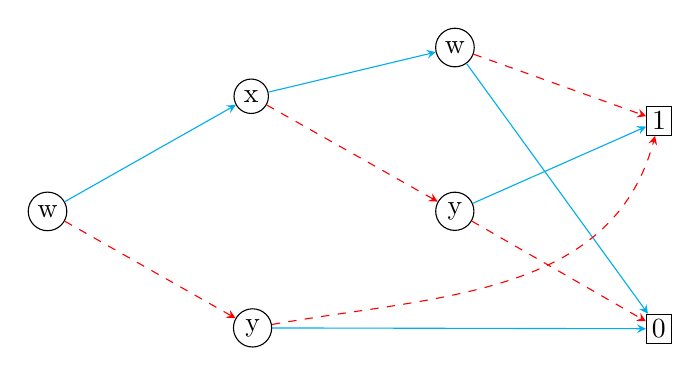
\begin{tikzpicture}[
node distance = 8pt and 64pt,
inner/.style={circle, draw=black, inner sep = 2pt, minimum size = 2pt},
terminal/.style={rectangle, draw=black, inner sep = 2pt, minimum size=2pt},
low/.style ={-stealth,dashed,red},
high/.style = {-stealth, solid,cyan}]

\node[inner] (0c0) {w};
\node[inner] (1c0) [above right = 32pt and 64pt of 0c0] {x};
\node[inner] (1c1) [below right = 32pt and 64pt of 0c0] {y};
\node[inner] (2c0) [above right = of 1c0] {w};
\node[inner] (2c1) [below right = 32pt and 64pt of 1c0] {y};

\node[terminal] (1) [below right = 16pt and 64pt of 2c0] {1};
\node[terminal] (0) [below right = 32pt and 64pt of 2c1] {0};

\draw[high](0c0)--(1c0);
\draw[low](0c0)--(1c1);
\draw[high](1c0)--(2c0);
\draw[low](1c0)--(2c1);

\draw[high](2c0)--(0);
\draw[low](2c0)--(1);
\draw[high](2c1)--(1);
\draw[low](2c1)--(0);

\draw[high](1c1)--(0);
\draw[low](1c1) to[out=10, in=255] (1);
\end{tikzpicture}
\end{center}
\end{example}
\end{frame}

\subsection[Size]{Size}
\begin{frame}
\frametitle{BDD size}
The \textit{size} of a BDD is its number of vertices.
\begin{example}
The following BDD has size $4$:
\begin{center}
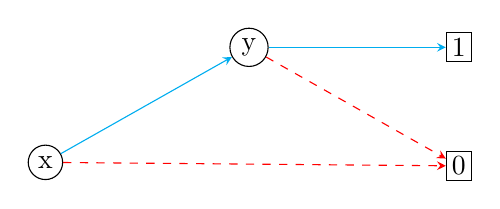
\begin{tikzpicture}[
node distance = 32pt and 64pt,
inner/.style={circle, draw=black, inner sep = 2pt, minimum size = 2pt},
terminal/.style={rectangle, draw=black, inner sep = 2pt, minimum size=2pt},
low/.style ={-stealth,dashed,red},
high/.style = {-stealth, solid,cyan}]

\node[inner] (0c0) {x};
\node[inner] (1c0) [above right = of 0c0] {y};

\node[terminal] (1) [right = of 1c0] {1};
\node[terminal] (0) [below = of 1] {0};

\draw[high](0c0)--(1c0);
\draw[high](1c0)--(1);
\draw[low](0c0)--(0);
\draw[low](1c0)--(0);
\end{tikzpicture}
\end{center}
\end{example}
\end{frame}

%\subsection[Successors]{Successors}
%\begin{frame}
%\frametitle{Successors}
%In a BDD, a node $y$ is the \textit{low-successor} of a nonterminal node $x$ if there is a low edge incident from $x$ to $y$. Similarly, $y$ is the \textit{high-successor} of $x$ if there is a high edge incident from $x$ to $y$.
%\end{frame}

\subsection[OBDD]{OBDD}
\begin{frame}
\frametitle{OBDD}
A BDD is \textit{ordered} (OBDD) if all paths from its root to a terminal node respect a given linear order on its variable labels. 
\end{frame}

\begin{frame}
\begin{example}
\begin{description}
\item [Function:] $f(w,x,y,z) = w \oplus x \oplus y \oplus z $\\
\item [Order:] $w<x<y<z$
\end{description}
\begin{center}
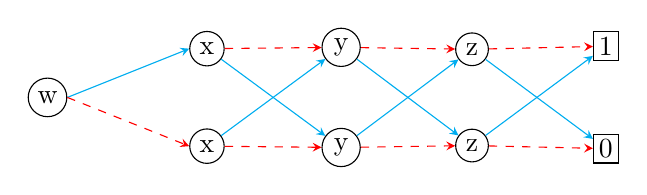
\begin{tikzpicture}[
node distance = 8pt and 32pt,
inner/.style={circle, draw=black, inner sep = 2pt, minimum size = 2pt},
terminal/.style={rectangle, draw=black, inner sep = 2pt, minimum size=2pt},
low/.style ={-stealth,dashed,red},
high/.style = {-stealth, solid,cyan}]

\node[inner] (0c0) {w};
\node[inner] (1c0) [above right = 8 pt and 48pt of 0c0] {x};
\node[inner] (1c1) [below right = 8 pt and 48pt of 0c0] {x};
\node[inner] (2c0) [above right = 8 pt and 96pt of 0c0] {y};
\node[inner] (2c1) [below right = 8 pt and 96pt of 0c0] {y};
\node[inner] (3c0) [above right = 8 pt and 144pt of 0c0] {z};
\node[inner] (3c1) [below right = 8 pt and 144pt of 0c0] {z};
\node[terminal] (1) [above right = 8 pt and 192pt of 0c0] {1};
\node[terminal] (0) [below right = 8 pt and 192pt of 0c0] {0};
\draw[high](0c0.east)--(1c0.west);
\draw[low](0c0.east)--(1c1.west);

\draw[low](1c0)--(2c0);
\draw[high](1c0)--(2c1);
\draw[high](1c1)--(2c0);
\draw[low](1c1)--(2c1);

\draw[low](2c0)--(3c0);
\draw[high](2c0)--(3c1);
\draw[high](2c1)--(3c0);
\draw[low](2c1)--(3c1);

\draw[low](3c0)--(1);
\draw[high](3c0)--(0);
\draw[high](3c1)--(1);
\draw[low](3c1)--(0);
\end{tikzpicture}
\end{center}
\end{example}
\end{frame}

\begin{frame}
In an OBDD,
\begin{itemize}
\item Every path from the root to a $1$-labeled terminal node corresponds to an assignment for which the corresponding boolean function evaluates to $1$.
\item Every path from the root to a $0$-labeled terminal node corresponds to an assignment for which the corresponding boolean function evaluates to $0$.
\end{itemize}
\end{frame}

\subsection[Construction]{Construction}
\begin{frame}
\begin{example}[Construction]
\begin{description}
\item [Function:] $f(w,x,y,z) = wx \oplus yz $\\
\item [Order:] $w<x<y<z$
\end{description}
\begin{tikzpicture}[
node distance = 48pt and 48pt,
inner/.style={circle, draw=black, inner sep = 2pt, minimum size = 2pt},
terminal/.style={rectangle, draw=black, inner sep = 2pt, minimum size=2pt},
low/.style ={-stealth,dashed,red},
high/.style = {-stealth, solid,cyan}]

\onslide<1->{\node[inner,onslide={<1,2,3>{highlight}}, label= left: {\onslide<-18>{\small $wx \oplus yz$}}] (0c0) {w};}
\onslide<2->{\node[inner,onslide={<4,5,6>{highlight}}, label= above: {\onslide<-18>{\small $x \oplus yz$}}] (1c0) [above right = 24pt and 48pt of 0c0] {x};}
\onslide<5->{\node[inner,onslide={<10,11,12>{highlight}}, label= below: {\onslide<-18>{\small $1 \oplus yz$}}] (2c0) [right = of 1c0] {y};}
\onslide<3->{\node[inner,onslide={<7,8,9>{highlight}}, label= above: {\onslide<-18>{\small $yz$}}] (2c1) [below = of 2c0] {y};}
\onslide<11->{\node[inner,onslide={<16,17,18>{highlight}},onslide={<19>{inner}}, label= above: {\onslide<-18>{\small $1 \oplus z$}}] (3c0) [right = of 2c0] {z};}
\onslide<8->{\node[inner,onslide={<13,14,15>{highlight}}, label= below: {\onslide<-18>{\small $z$}}] (3c1) [below = of 3c0] {z};}
\onslide<12->{\node[terminal,label= above: {\onslide<-18>{\small $1$}}] (1) [right = of 3c0] {1};}
\onslide<9->{\node[terminal,label= below: {\onslide<-18>{\small $0$}}] (0) [below = of 1] {0};}

\onslide<2->{\draw[high](0c0)--(1c0);} %d
\onslide<5->{\draw[high](1c0)--(2c0);} %d
\onslide<6->{\draw[low](1c0) to[out=310, in=140] (2c1);} %d
\onslide<3->{\draw[low](0c0) to[out=330, in=180] (2c1);} %d
\onslide<11->{\draw[high](2c0)--(3c0);} %d 8
\onslide<8->{\draw[high](2c1)--(3c1);} %d 6
\onslide<12->{\draw[low](2c0) to[out=45, in 135] (1);} %d 9
\onslide<9->{\draw[low](2c1) to[out=315, in=225] (0);} %d 7
\onslide<17->{\draw[high](3c0)--(0);} %d 12
\onslide<18->{\draw[low](3c0)--(1);} %d 13
\onslide<14->{\draw[high](3c1)--(1);} %d 10
\onslide<15->{\draw[low](3c1)--(0);} %d 11
\end{tikzpicture}
\end{example}
\end{frame}

%\subsection[ROBDD]{ROBDD}
%\begin{frame}
%\frametitle{ROBDD}
%An OBDD is \textit{reduced} (ROBDD) if no node has identical low- and high-successors, and no two distinct nodes have the same variable names and low- and high-successors where if two distinct nodes both lack a low-successor (high-successor) then they are considered to have identical low-successors (high-successors).
%\end{frame}

%\begin{frame}
%\begin{example}
%An ROBDD in the variables $w,x,y,z$ using ordering $w<x<y<z$,
%\end{example}
%\end{frame}

\section[Fact to BDD SAT]{FACT to BDD SAT}
\begin{frame}
\frametitle{FACT to BDD SAT}
\begin{itemize}
\item Each of the $f_m$ making up $F_a$ can be represented by an OBDD.
\item In 2005 Philipp Woelfel showed that regardless of the linear order used, $f_{n-1}$ will have size greater than $2^{\lfloor n/2 \rfloor}/61-4$ \cite{Woel/2005}.
\item Using $F_a$ as defined previously results in an exponential size representation.
\item Conclusion: using $F_a$ as previously defined is infeasible.
\end{itemize}
\end{frame}


\subsection[Proceed]{Proceed}
\begin{frame}
\frametitle{How to proceed?}
Find an equivalent function (system) to $F_a$ ($S_a$) and corresponding replacements for each $1 \oplus a_m \oplus f_m$ with smaller OBDD representations.
\pause
\checkmark
\end{frame}

\begin{frame}
Replacement for each $1 \oplus a_m \oplus f_m$, $g_m$, has an OBDD size of less than $6(2n)^3$. This results in a replacement for $F_a$, $G_a$, with a BDD representation of polynomial size $O(n^4)$.
\end{frame}

\subsection[Problem]{Problem}
\begin{frame}
\frametitle{Problem}
The linear order used for each $g_m$ is not the same.
\end{frame}

\begin{frame}
To extract a factorization of $a$ from the BDD, we must find a path from the root to the $1$-terminal node such that in the path 
\begin{enumerate}
\item We never leave a node with a label $t$ along a $0$ edge and then later leave another node with the same label $t$ along a $1$ edge.
\item We never leave a node with a label $t$ along a $1$ edge and then later leave another node with the same label $t$ along a $0$ edge.
\end{enumerate}
\end{frame}

\subsection[Future work]{Future work}
\begin{frame}
\frametitle{Open questions and directions for future work}
\begin{itemize}
\item Compare other normal form representations besides BDDs for $G_a$ to $F_a$.
\item Compare the performance of some CNF SAT solvers on CNF SAT instances obtained from $G_a$ to those obtained from $F_a$.
\item Check the performance of some BDD-based SAT solving algorithms on $G_a$.
\end{itemize}
\end{frame}

\section[References]{References}
\begin{frame}[allowframebreaks]
\frametitle{References}
\bibliography{thebib}
\bibliographystyle{ieeetr}
\end{frame}
\end{document}
